\documentclass[letter,11pt]{article}

\usepackage[spanish,es-nodecimaldot]{babel}
\usepackage[utf8]{inputenc}

\usepackage{lmodern}
\usepackage[T1]{fontenc}
\usepackage{textcomp}

\usepackage{framed}
\usepackage[svgnames]{xcolor}
\colorlet{shadecolor}{Gainsboro!50}

\usepackage{enumitem}
\usepackage{graphicx}
\usepackage{pstricks}

\usepackage{anysize}
\marginsize{3cm}{2cm}{2cm}{3cm}

\usepackage{siunitx}
\usepackage{amsmath}
\usepackage{array}
\usepackage{alltt}

\usepackage{fancyhdr}
\usepackage{lastpage}
\pagestyle{fancy}
\fancyhf{}
\fancyhead[LE,RO]{Mecánica de fluidos}
\fancyfoot[CO,CE]{\thepage\ de \pageref{LastPage}}

\special{papersize=215.9mm,279.4mm}

\usepackage[
    pdfauthor={Carlos Eduardo Caballero Burgoa},%
    pdftitle={Mecánica de fluidos},%
    pdfsubject={Practica 01},%
    colorlinks,%
    citecolor=black,%
    filecolor=black,%
    linkcolor=black,%
    urlcolor=black,
    breaklinks]{hyperref}
\usepackage{breakurl}

\newcommand{\blankpage}{
\newpage
\thispagestyle{empty}
\mbox{}
\newpage
}

\renewcommand{\arraystretch}{1.2}

\begin{document}

\begin{center}
    {\large \bf{\underline{Practica \#01}}}
\end{center}
\vspace{0.25cm}

\begin{enumerate}
\item \textbf{Un espacio anular entre los cilindros concentricos con una
longitud en contacto de $0.15 m$, esta llena de glicerina
($\mu=\num{4.1e{-1}} N\,s/m^2$). Los diametros de los cilindros interno y
externo son: $152.4 mm$ y $157.5 mm$ respectivamente. Determine el torque y la
potencia necesaria para mantener girando al cilindro interno a $180 rpm$.}

\begin{figure}[!h]
\centering
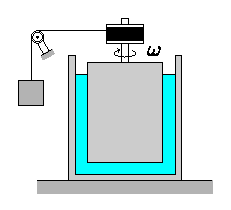
\includegraphics[scale=1.35]{figura01.eps}
\end{figure}

\item \textbf{El diametro y la altura del cilindro mostrado en la figura son
$204 mm$ y $305 mm$ respectivamente. Observe que el objeto se desliza sobre un
aceite de espesura constante que esta en el plano inclinado, su viscosidad es
$\mu=\num{9.6e{-1}} N\,s/m^2$ sabiendo que la masa del cilindro es de $18.14 kg$
determinar el angulo del plano inclinado.}

\begin{figure}[!h]
\centering
\includegraphics[scale=1.50]{figura02.eps}
\end{figure}

\item \textbf{Desarrolla una expresion para la viscosidad si se asume como dato
conocido el torque.}

\begin{figure}[!h]
\centering
\includegraphics[scale=2.00]{figura03.eps}
\end{figure}

\item \textbf{Para el conjunto de masas mostradas en la figura. Determinar una
expresion para la velocidad en funcion del tiempo ($V(t)$). Si la masa $M$ se
desliza sobre un fluido de viscosidad $mu$ y el espesor $e$. Considerar $A$ como
el area en contacto y el valor de las masas $M$ y $m$ respectivamente como se
muestra en la figura.}

\begin{figure}[!h]
\centering
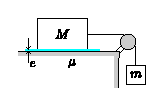
\includegraphics[scale=2.00]{figura04.eps}
\end{figure}

\end{enumerate}

\end{document}
